% Internal paper draft. The original cumulative report remains in main.tex/named.pdf.
\documentclass[sigconf,dvipsnames]{acmart}
\setcopyright{none}
\settopmatter{printacmref=false,printfolios=true}
\acmDOI{}
\acmISBN{}
\acmConference[Research draft]{Internal supervisor discussion draft}{19 October 2026}{}
\usepackage{algorithm}
\usepackage{algpseudocode}
\usepackage{xurl}
\setlength{\emergencystretch}{2em}
\graphicspath{{../../figures/ManiGuard/phase3-recovery/}{../../figures/ManiGuard/phase3-part1/}}
\newcommand{\ind}{\mathbf{1}}
\newcommand{\safe}{S_{\mathrm{req}}}
\newcommand{\complete}{C_{\mathrm{req}}}
\newcommand{\disabled}{\varnothing}
\begin{document}
\title{Intervention-Aware Execution Adaptation around Frozen Manipulation Policies}
\subtitle{Evolutionary selection, feedback timing and a direction-preserving recovery diagnostic}
\author{Sachin Mohan}
\affiliation{\institution{University of the Witwatersrand}\city{Johannesburg}\country{South Africa}}
\email{2699183@students.wits.ac.za}
\renewcommand{\shortauthors}{Mohan}
\begin{abstract}
Can a compact execution controller improve safe completion around a frozen
vision-language-action policy under a small interaction budget? We study joint-target
restraint and policy-query timing in ManiGuard Clutter, retaining the native task and
safety monitors. A 24-episode evolutionary search selects a four-gene controller;
24 subsequent comparison episodes reveal 4/8 safe completions and 2/8 violations at
full strength, against identity's 5/8 and 0/8. A separate sixteen-episode feedback
pilot finds no early activation of its correction trigger. We then implement a uniform,
direction-preserving cap and evaluate it on 18,657 saved commands from 24 historical
episodes. At 0.04 rad, componentwise clipping distorts joint-error direction by more
than five degrees on 9/55 modified commands; vector scaling does so on 0/55. A frozen
median correction threshold admits three early-query opportunities in 482 diagnostic
prefixes, with sparse calibration support. This is an offline mechanism result, not
a demonstrated physical safety gain. Supporting forecast and warning-prediction
audits explain why model-assisted search remains untested. The study identifies
specific implementation repairs and the controlled comparison needed to distinguish
an execution benefit from an evolutionary-search benefit.
\end{abstract}
\begin{CCSXML}
<ccs2012><concept><concept_id>10010147</concept_id>
<concept_desc>Computing methodologies</concept_desc>
<concept_significance>500</concept_significance></concept></ccs2012>
\end{CCSXML}
\ccsdesc[500]{Computing methodologies}
\keywords{evolutionary robotics, frozen policies, execution adaptation, safe manipulation}
\maketitle

\section{Introduction}
A manipulation policy can complete a task while tipping a protected object or
violating another physical requirement. Conversely, a controller can avoid a
violation by doing little and leaving the task unfinished. ManiGuard makes this
distinction explicit through independent task checks and runtime monitors over
physics-grounded predicates~\cite{maniguard}. This makes safe completion, violations
and unfinished episodes necessary companion outcomes.

Our question is whether a small controller around a frozen policy can improve this
trade-off with substantially less adaptation machinery than training the underlying
policy. The controller changes arm-target magnitude and the frequency of observation
feedback. Evolution searches its categorical parameters using complete simulator
episodes. An external dial interpolates between the original policy and the selected
controller. A useful result would require improved measured safe completion, a
credible physical-violation comparison, and an advantage that survives matched random
search and ordinary learning.

The completed evidence has a more limited outcome. The first evolutionary finalist
does not improve the subsequent comparison. The second pilot does not activate its
adaptive timing mechanism. These observations motivate a repair with a precise
software property: preserve the proposed joint-error direction when limiting target
displacement. The new saved-trace experiment verifies that property and measures how
rarely a correction-based refresh could have acted on the available records.

The paper contributes an implemented execution interface, an audited small-budget
study with adverse and null results, and a reproducible diagnostic linking a concrete
geometry repair to its remaining physical test. It does not establish optimizer
superiority, a calibrated safety dial, or a safety guarantee. This internal draft
consolidates completed work and explicitly identifies the unexecuted comparisons.

\begin{figure*}[t]
\centering
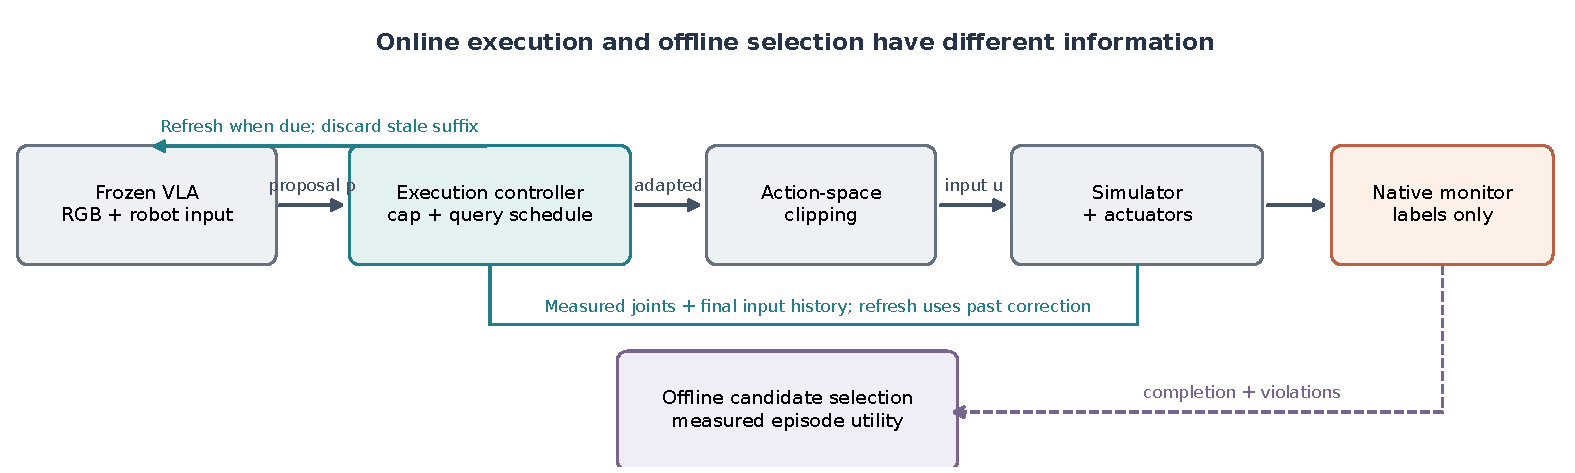
\includegraphics[width=.98\textwidth]{architecture.pdf}
\caption{Information flow. The execution controller receives policy proposals,
measured robot state and past final environment inputs. Native monitor outcomes enter
offline evaluation and candidate selection. The monitor does not veto or replace an
action. Final environment input precedes lower-level actuator processing.}
\Description{A frozen VLA proposes actions to an execution controller, followed by
action-space clipping and simulation. Robot feedback returns to the controller.
The monitor labels outcomes for offline selection.}
\label{fig:architecture}
\end{figure*}

\section{Context and research question}
ManiGuard supplies specification-grounded manipulation tasks and separates success
from safety~\cite{maniguard}. We use its frozen Clutter policy and pinned openpi
implementation~\cite{openpi}; we do not train a new VLA. Our adapter has no online
access to protected-object poses, native grasp labels or monitor predicates.

Dynamics models can reduce the physical evaluations needed for skill
search~\cite{daqd}. Frozen visual representations also support learned dynamics
and planning~\cite{dinov2,dinowm}, while model-based policy optimization motivates
testing where predictions remain useful~\cite{mbpo}. These precedents make a new
optimizer name or the use of visual features insufficient as a novelty claim.
Our proposed contribution concerns execution intervention and the allocation of
limited physical evaluations. The current study first asks whether the execution
mechanism works, and separately whether the predictive prerequisites are adequate.

We distinguish three questions: does the execution map improve outcomes over identity;
does adaptive refresh contribute beyond a fixed schedule; and does evolutionary
selection improve over other adaptation methods at matched cost? The completed
pilots address the first two only in a small descriptive sample. The third remains
open because matched random-search and ordinary-learning arms have not run.

\section{Problem and evaluation boundary}
At policy query time $\tau$, a frozen policy produces a sequence
$P_\tau=\pi(o_\tau;\xi)$ from two RGB views, native robot input and its task prompt.
Between queries, the controller consumes cached proposals $p_t\in\mathbb R^8$.
Their first seven coordinates are arm joint targets and the eighth is the gripper
proposal after native binarization. Measured arm joints are $q_t\in\mathbb R^7$.
The adapter produces $a_t$ and native action-space clipping produces the final
environment input $u_t$. We log $p_t$, $a_t$ and $u_t$ separately. The simulator's
actuator processing is a further boundary; a bound on $u_t-q_t$ is not a bound on
joint speed, contact force, end-effector motion or object tilt.

Let $V$ be the episode's native raw \texttt{ltl\_violated} flag. Requested completion
$\complete$ combines native success with the pinned Clutter completion checklist.
Safe completion and the training utility are
\begin{equation}
 \safe=\complete\land\neg V,\qquad
 U=\ind(\safe)-2\ind(V).
 \label{eq:utility}
\end{equation}
Thus a violating episode receives $-2$, an unfinished nonviolating episode receives
zero, and a safe completion receives one. This is a declared penalized utility.
It is not penalty-free optimization. Reporting retains the four joint categories:
safe completion, unsafe completion, safe unfinished and unsafe unfinished.

The monitor labels consequences and never changes commands
(Figure~\ref{fig:architecture}). Throughout this draft, ``execution controller''
refers to our map and query scheduler. There is no learned online safety filter,
world-model veto or ROSARL integration in the executed system.

\section{Methodology}
\subsection{Original categorical execution controller}
Part 1 searches $\theta=(c_f,c_g,\alpha,h)$ over
\begin{align}
 c_f&\in\{\disabled,.12,.08,.04\}\ \mathrm{rad}, &
 c_g&\in\{\disabled,.08,.04,.02\}\ \mathrm{rad},\nonumber\\
 \alpha&\in\{1,.75,.5\}, &h&\in\{4,8,16\}.
\end{align}
The domain contains 144 genotypes. At the first action $r_t=q_t$; subsequently
$r_t=u_{t-1}^{\rm arm}$. The anchor computes
\begin{equation}
 z_t=r_t+\alpha(p_t^{\rm arm}-r_t),\quad
 a_t^{\rm arm}=q_t+\operatorname{clip}(z_t-q_t,-c,c),
 \label{eq:component}
\end{equation}
or $a_t^{\rm arm}=z_t$ when the selected cap is disabled. The gripper proposal is
preserved. A fixed causal heuristic chooses $c_g$ when both absolute finger positions
are in $[.003,.035]$ m, maximum finger change is below .002 m, and the current proposal
closes the gripper. Otherwise it chooses $c_f$. This heuristic is robot evidence
rather than a held-object detector.

An episode-constant dial $d\in[0,1]$ applies
\begin{equation}
 \widetilde a_t^{\rm arm}=p_t^{\rm arm}+d(a_t^{\rm arm}-p_t^{\rm arm}),\quad
 h(d)=\left\lfloor8+d(h-8)+.5\right\rfloor.
\end{equation}
At zero, an explicit bypass returns the original proposal bitwise. At one, the
anchor is returned directly. The experiment searches at $d=1$ and evaluates the
frozen finalist at $d\in\{0,.5,1\}$. Native gripper handling, goals, monitor rules
and early success termination remain unchanged.

\subsection{Evolution with fresh elite evaluation}
Algorithm~\ref{alg:evolution} gives the executed Part 1 search. PCG64 seed 20261018
initializes identity and three distinct uniform random genotypes. Each population
has four candidates, each evaluated on two training cases. After stable ranking
by mean utility, the best two candidates become parents. The next population
physically re-evaluates the best parent and evaluates three new children; historical
elite fitness is never copied into a new generation.

\begin{algorithm}[t]
\caption{Executed Part 1 evolutionary search}
\label{alg:evolution}
\begin{algorithmic}[1]
\Require Frozen policy, domain $\Theta$, sealed cases and seeds
\State $P_0\gets$ identity plus three distinct uniform points
\For{$g=0,1,2$}
  \For{candidate $\theta_i$ in $P_g$}
    \State Run two fresh full simulator episodes at dial one
    \State Audit both records; set $F_i\gets(U_{i,1}+U_{i,2})/2$
  \EndFor
  \State Rank by decreasing $F_i$, then stable birth order
  \If{$g<2$}
    \State Retain top two parents; copy best into $P_{g+1}$
    \State Add three distinct categorical mutants of those parents
  \EndIf
\EndFor
\State Freeze best candidate in the final evaluated population
\State Evaluate its three dial settings on eight matched blocks
\Ensure Full lineage, all outcomes and all interaction costs
\end{algorithmic}
\end{algorithm}

Mutation selects one of the two parents uniformly and designates one coordinate
for mutation. Each other coordinate is visited with probability .5. A visited
coordinate is uniformly resampled with probability .2; otherwise its index moves
by one of $\{-2,-1,1,2\}$ and is clipped to the categorical range. Rejection removes
unchanged offspring and duplicates within the new population. After at most 100
draws, a declared uniform fallback selects an unused eligible point. These are
index operations on the declared domain, not Gaussian mutations of physical units.
Invalid infrastructure records have no fitness and cannot enter ranking.

Only the final evaluated population supplies the finalist. Search uses tasks
0034/0002, with seed $1000+10g+i$ for task index $i$. The 24 comparison episodes
use tasks 0029/0032, four repetitions each, at all three dial settings. Their seeds
are $2000+10j+r$. A separate schedule RNG interleaves conditions within blocks.
These scenes are conservatively considered exposed; the comparison supplies fresh
repetitions rather than new-task transfer evidence.

\subsection{Correction-aware feedback scheduling}
Part 2 removes smoothing and the long sixteen-action interval, retains the finalist's
.04/.02 rad caps, and compares identity/8 (A), cap/8 (B), cap/4 (C), and adaptive
cap/4--8 (D). The adaptive scheduler accumulates normalized departure between
the proposal and the final environment input:
\begin{equation}
 D_k=\sum_{t=\tau}^{\tau+k-1}
 \frac{\|\mathcal T(p_t^{\rm arm}-u_t^{\rm arm})\|_2}{\sqrt7\,(.04\ \mathrm{rad})},
 \label{eq:correction}
\end{equation}
where $\mathcal T$ zeros per-coordinate differences no larger than $10^{-6}$ rad.
The sum uses already applied inputs, includes downstream clipping and resets at
each policy query. Finger history persists. With minimum interval four, D queries
when $D_k\ge.5$ or at maximum age eight, subject to native termination taking
precedence. A zero threshold is a fixed-frequency reference; a disabled threshold
is fixed-eight execution. Correction measures command departure, not physical risk.

\begin{algorithm}[t]
\caption{Causal correction-aware execution interface}
\label{alg:feedback}
\begin{algorithmic}[1]
\State Reset accumulated correction and cached policy prefix
\While{episode has not terminated}
  \If{no prefix, prefix exhausted, or refresh is due}
    \State Query frozen policy at current observation
    \State Discard old suffix; reset $D\gets0$, $k\gets0$
  \EndIf
  \State Read next proposal $p_t$ and measured joints $q_t$
  \State $a_t\gets$ declared cap map; preserve gripper
  \State $u_t\gets$ native action-space clipping of $a_t$
  \State Apply $u_t$; log proposal, adaptation and final input
  \State Update $D$ using Eq.~\eqref{eq:correction}; $k\gets k+1$
  \State Refresh due if $k=8$ or $(k\ge m\land D\ge\eta)$
\EndWhile
\end{algorithmic}
\end{algorithm}

The sixteen-episode schedule uses two repetitions of tasks 0039/0010 and rotates
ABCD, BCDA, CDAB and DABC across four blocks. It is a separate feedback pilot,
not a new evolutionary search. The same passive observation capture runs in all
conditions. No trigger threshold is retuned during that physical comparison.

\subsection{Uniform direction-preserving recovery map}
The new recovery implementation fixes smoothing to one and removes grasp conditioning.
For joint-error vector $e_t=p_t^{\rm arm}-q_t$, define
\begin{equation}
 s_t=\begin{cases}
 1,&\|e_t\|_\infty=0,\\
 \min(1,c/\|e_t\|_\infty),&\text{otherwise},
 \end{cases}
 \qquad a_t^{\rm arm}=q_t+s_te_t.
 \label{eq:radial}
\end{equation}
For $c>0$, scalar multiplication preserves the joint-error direction and bounds
every coordinate's target error by $c$ before numerical rounding. Componentwise
clipping can rotate that direction when coordinates saturate differently
(Figure~\ref{fig:geometry}). This property concerns joint-space targets. It does
not preserve Cartesian motion or certify collision avoidance or uprightness.
Downstream clipping and actuator processing can alter the physical interpretation.
The disabled branch returns the original proposal exactly.

\begin{figure}[t]
\centering
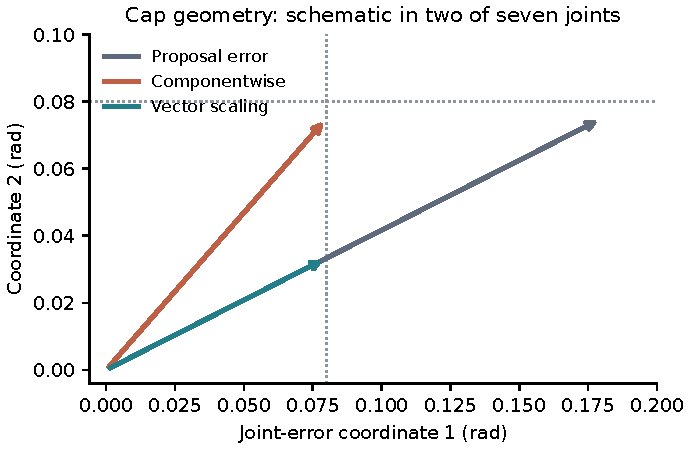
\includegraphics[width=\linewidth]{geometry-schematic.pdf}
\caption{A schematic of the two cap maps. Both limit the largest joint-error
coordinate; uniform scaling retains the original error direction. This is a
two-coordinate illustration, not a simulated or measured robot trajectory.}
\Description{Three vectors show the original joint error, a rotated componentwise
cap, and a collinear scaled error.}
\label{fig:geometry}
\end{figure}

The saved-trace protocol fixes disabled/.12/.08/.04 rad caps and evaluates both maps
on all 24 verified full Part 2/3 recordings. Every proposal is transformed at its
factual measured joints, preserving its recorded dtype and gripper. We replay the
recorded action-space bounds and measure direction before and after that boundary.
Engineering episodes are excluded. None of these alternate inputs is executed.

For the timing diagnostic, the cap is fixed at .04 rad before scoring. Calibration
uses the eight B/D episodes on tasks 0010/0039. Only complete factual eight-action
prefixes are eligible. We collect strictly positive accumulated correction at ages
four through seven and derive thresholds from their .50/.75/.90 quantiles. The
median is the prospectively selected reference. A diagnostic panel uses only the
four fixed-eight B recordings on tasks 0046/0006, excluding four-action schedules
and incomplete final prefixes. Both minimum intervals four and six are reported.
All four tasks were exposed previously, so this panel is development evidence,
not a fresh recovery audit.

\begin{algorithm}[t]
\caption{Saved-trace trigger-opportunity diagnostic}
\label{alg:replay}
\begin{algorithmic}[1]
\Require Verified records, fixed cap, calibration/diagnostic tasks
\For{each complete factual eight-action calibration prefix}
  \State Map saved $p_t,q_t$ with Eq.~\eqref{eq:radial}; apply saved bounds
  \State Compute cumulative correction using these mapped inputs
  \State Collect positive $D_k$ for $k\in\{4,5,6,7\}$
\EndFor
\State Freeze the declared three quantile thresholds
\For{each complete factual eight-action diagnostic prefix}
  \State Find first $k\in\{m,\ldots,7\}$ with $D_k\ge\eta$
  \State Count one opportunity if such $k$ exists
  \State Make no claim about proposals after that hypothetical query
\EndFor
\Ensure Opportunity counts, support, task denominators and zero new physics
\end{algorithmic}
\end{algorithm}

The first would-trigger age is an open-loop diagnostic within a factual prefix.
After that point a real policy query would produce new proposals and a different
trajectory. We therefore infer neither counterfactual completion nor total new
query cost from this replay. Threshold support and per-task activation are reported
alongside pooled counts.

\subsection{Supporting prediction audits}
Part 3 separately tests whether a compact predictive system is useful enough to
help allocate evolutionary evaluations. A frozen DINOv2-small encoder supplies
$2\times2$ spatially pooled features from two cameras, 3,072 coordinates
in total~\cite{dinov2}. Fitting-only standardization and PCA retain 32 visual
coordinates; arm joints and fingers remain separate. Five episode-bootstrap
128/128-unit residual MLPs predict standardized visual/robot changes from current
and previous state plus previous/current executed inputs. Training is fixed at
30 epochs. Causal histories shift during rollouts of at most four actions.

Ridge readouts predict upright margin and negative target-to-goal distance. The
audit separates readout error on actual future states from error after predicted
dynamics. References include persistence, ridge and shuffled-action tests.
Disagreement-only trust and a correction-conditional factual-error rule are compared
before any physical use. Object-state targets are evaluation labels and never
become online controller inputs. A distance readout is distinct from native held
completion; a tilt readout is distinct from spill or drop safety.

Part 4 instead fits a direct warning predictor for the first native uprightness
event within eight actions, with a warning deadline four actions before onset.
Its causal inputs include current visual features, robot/proposal history, four
past executed inputs, controller metadata and query age. A five-member 64-unit
MLP ensemble uses 500 updates per member; logistic and visual-only references are
retained. Probability and alarm rules calibrate on a separate task at natural
prevalence with episode weights. This is a warning-classification audit, not a
repaired latent world model or an executed counterexample search.

\section{Experimental protocol and accounting}
All physical episodes use the pinned ManiGuard Clutter setup, two $256\times256$
camera inputs, native gripper binarization, assisted grasping, raw joint control,
20 Hz action/render and 120 Hz physics. The frozen checkpoint is step 7100 at
revision \texttt{f572e33bdb49}; the full revision and file hashes remain in the
controller export. The native horizon is 1,100 policy actions, with native early
termination. No episode is shortened to obtain a favourable completion count.

Historical physical execution used separate uv-managed Python 3.10 simulation
and Python 3.11 policy environments on one RTX 4090. The present check-in uses a
different RTX 4090 preparation machine without an installed ManiGuard stack. Its
new experiment is CPU replay of private revision-pinned recordings. It creates no
new physics, policy queries, encoder calls, fitted predictors or physical outcomes.

The original model partitions use sixteen Part 2 episodes for fitting, four task
0046 episodes for calibration and four task 0006 episodes for audit. Once exposed,
these tasks cannot become fresh recovery evaluation. The main-study test partition
remains excluded. All 24 historical acquisitions are charged once, including
discarded candidates and recording costs; reuse adds analysis cost rather than
new physical experience. Table~\ref{tab:ledger} retains the cumulative lower bounds.

\begin{table}[t]
\caption{Cumulative historical physical costs, counted once. Unknown initialization
physics and one pre-application failure prevent treating these as exact totals.}
\label{tab:ledger}
\begin{tabular}{lrrr}
\toprule
Stage & Attempts & Controls & VLA queries \\
\midrule
Part 1, all work & 52 & 35,158 & 3,401 \\
Part 2, all work & 20 & 11,286 & 1,796 \\
Part 3, recordings & 8 & 7,467 & 1,385 \\
Part 4, offline & 0 & 0 & 0 \\
New recovery replay & 0 & 0 & 0 \\
\midrule
Known physical total & 80 & 53,911 & 6,582 \\
\bottomrule
\end{tabular}
\end{table}

Matching task and sampling seed does not guarantee identical observations. All
sixteen Part 1 initial robot-state comparisons agree numerically, but both cameras
differ in every matched pair, and the first policy commands already differ before
adaptation. Part 2 likewise has equal initial robot states but different camera
images and first chunks. These checks prevent interpreting a single paired video
as an identified causal counterfactual.

\section{Results}
\subsection{Evolution selects a training winner that does not transfer}
The 24 search episodes evaluate twelve candidate measurements, including elite
re-evaluations. Five measurements attain maximum utility. The selected genome is
$[3,3,0,2]$: free cap .04 rad, grasp cap .02 rad, smoothing one and horizon sixteen.
It safely completes its two final training cases. The copied elite's fresh mean
score falls to .5. Two-case fitness is therefore visibly noisy, and the finalist's
perfect training score is not an estimate of general performance.

\begin{figure*}[t]
\centering
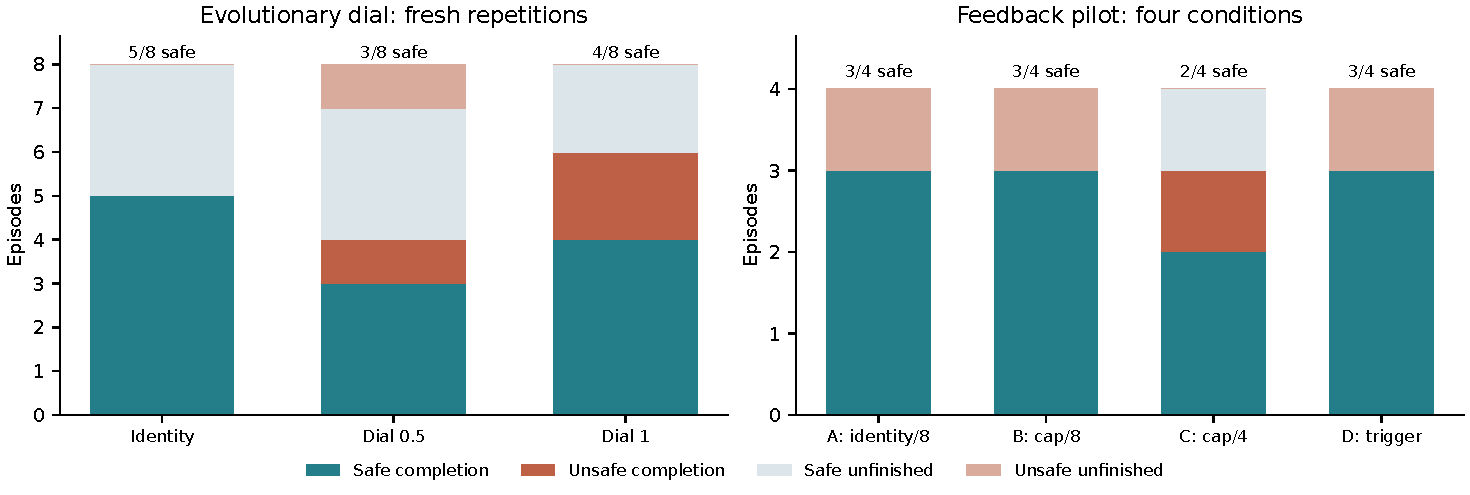
\includegraphics[width=.97\textwidth]{outcomes.pdf}
\caption{Every physical comparison outcome. Part 1 has eight repetitions per dial
setting across two scenes; Part 2 has four episodes per condition across two scenes.
All four completion/violation categories remain visible. These pilots do not
establish a superior controller or an optimizer advantage.}
\Description{Stacked bars show safe completions of five, three and four of eight in
Part 1, and three, three, two and three of four in Part 2, with violations retained.}
\label{fig:outcomes}
\end{figure*}

In the 24 subsequent comparison episodes, safe completion is 5/8 at identity, 3/8
at midpoint and 4/8 at full strength (Figure~\ref{fig:outcomes}). Violations are
0/8, 2/8 and 2/8. Full minus identity is a descriptive $-12.5$ percentage points
with two additional violating episodes. Full strength completes six requested
tasks, but two completions are unsafe. Its 312 queries are fewer than identity's
774; that resource saving accompanies worse measured safety and safe completion.
The altered query horizon and arm map are confounded in this pilot.

An exploratory failure audit identifies a grasp-heuristic gap: in one unsafe liquid
transport episode, it misses all 167 held-and-closing actions because a finger lies
outside the fixed band. Other safe episodes also contain misses, and both
obstacle-uprightness failures occur while the heuristic recognizes the grasp.
The gap is concrete but is not a sufficient causal explanation. A timeout likewise
does not distinguish inactivity, poor continuation, a restrictive controller or
insufficient horizon.

\subsection{The original adaptive trigger never refreshes early}
Identity, cap/8 and adaptive cap/4--8 each safely complete 3/4 episodes; cap/4
achieves 2/4. Each condition records one violation. All 337 observed inter-query
intervals for adaptive D are eight actions. Its sole .5-threshold crossing occurs
at action eight, when a query is already compulsory. There is no early crossing
at ages four through seven. This is a nonactivation result, not a comparison of
an active adaptive mechanism with a fixed scheduler.

Fixed-four uses 750 queries against fixed-eight's 336 without improving this small
sample's safe completion. This does not show that frequent feedback causes harm.
It does establish that assuming an efficiency benefit from more frequent queries
would be unsupported by the measured pilot.

\subsection{Recovery fixes command geometry, with sparse timing opportunity}
The new saved-trace screen uses 18,657 historical commands across 24 episodes on
four tasks. With a uniform .04 rad cap, both maps substantially change 55 commands.
Componentwise clipping rotates joint-error direction by more than $5^\circ$ on
9/55 changed commands, with maximum $10.32^\circ$. Vector scaling has 0/55 above
$5^\circ$ and maximum $0.00019^\circ$, consistent with float32 rounding. No saved
action-space bound further changes the arm command in this panel. Lower-level
actuator output limits are outside this replay.

\begin{figure*}[t]
\centering
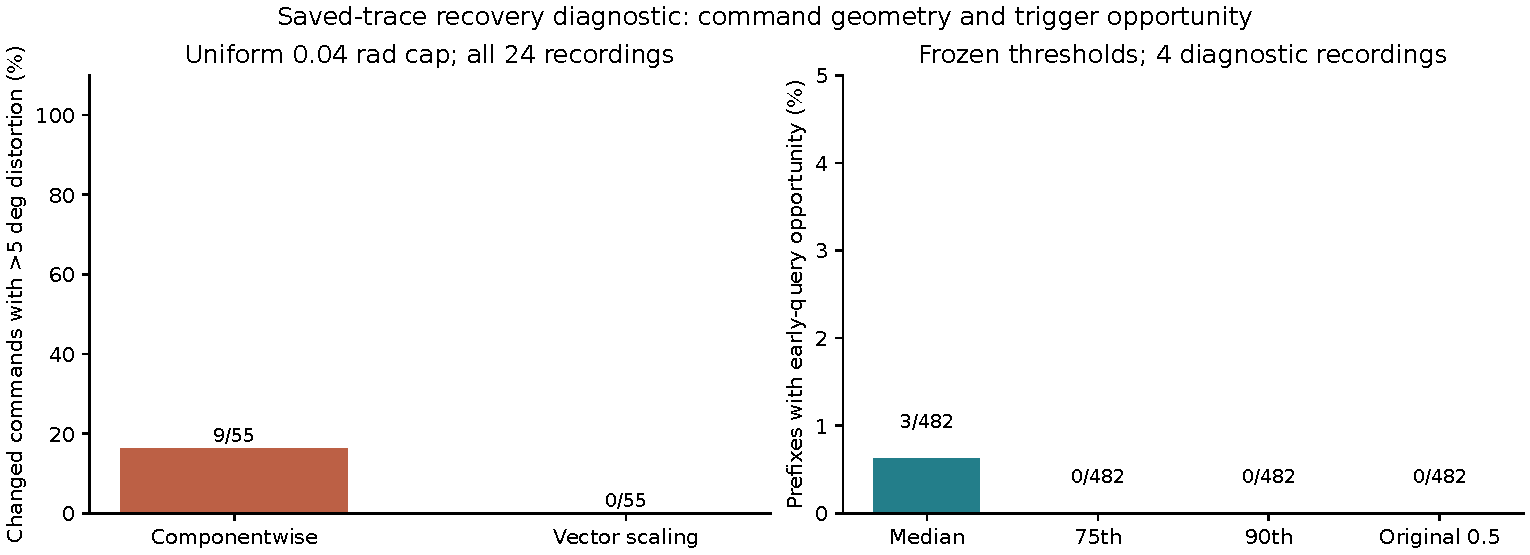
\includegraphics[width=.97\textwidth]{diagnostic.pdf}
\caption{New saved-trace diagnostic. Left: direction distortion conditional on a
substantially modified command at the .04 rad cap. Right: first early-query
opportunities in 482 complete factual eight-action diagnostic prefixes, using
thresholds frozen from calibration traces. Opportunity counts are neither actual
queries nor physical completion measurements. All tasks are previously exposed.}
\Description{Componentwise clipping distorts nine of fifty-five modified commands
by more than five degrees; vector scaling distorts none. The median threshold
admits three of 482 prefixes; the other thresholds admit none.}
\label{fig:diagnostic}
\end{figure*}

Only 55/18,657 commands, about .30\%, are substantially modified at .04 rad.
At .08 and .12 rad, the corresponding counts are three and one. These rates
describe proposals along the original trajectories. They do not establish how
often a deployed repaired controller would intervene after its states diverge.

Calibration has 669 complete eight-action prefixes but only five strictly positive
eligible accumulated-correction values. These correlated values yield thresholds
.089753, .536969 and .947503. The median threshold gives 3/482 early opportunities
on the diagnostic panel, present in two of four episodes and only task 0046.
The upper thresholds and original .5 reference give 0/482. This indicates a
possible timing opportunity with weak cross-task support. It does not justify a
claim of robust activation, saved query cost or improved physical safety.

The analysis completes in approximately eight CPU seconds after data restoration
and implementation. It performs zero new simulator controls, physics steps,
policy queries, encoder calls or trained-model fits. A repeated analysis after
lint/source-preservation cleanup produces identical geometry and timing tables;
both run receipts and source snapshots remain available. Twenty-one targeted
checks cover identity, finite inputs, dtype, cap geometry, downstream clipping,
causal correction, query reset and the age-eight boundary.

\subsection{Prediction prerequisites remain unsupported}
Part 3's four-action latent prediction error is 45.1\% worse than persistence.
The actual-state uprightness readout already has $16.17^\circ$ mean absolute
error, before model rollout; near-threshold predicted-state error is
$18.56^\circ$. All correction calibration lies in one supported bin, so the
correction-dependent trust mask equals the disagreement-only mask. The planned
64-episode model-assisted optimizer comparison is unstarted. Failed readout,
failed dynamics and indistinguishable selection rules are separate findings.

Part 4's frozen direct warning predictor alarms on 2,045/2,229 negative development
windows, or 91.75\%. Development contains one first-event episode and no confident
miss. The event support and operating point fail the premise for its conditional
physical acquisition design. No evolutionary counterexample-acquisition outcome,
diversity effect or predictor-repair benefit is claimed.

\begin{figure}[t]
\centering
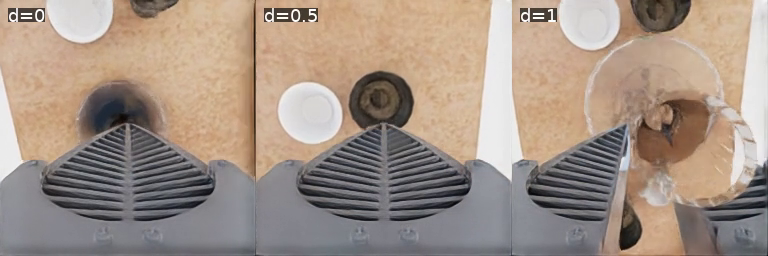
\includegraphics[width=\linewidth]{frames/task_0029-base-seed2000-wrist-t18s.png}\par
\smallskip
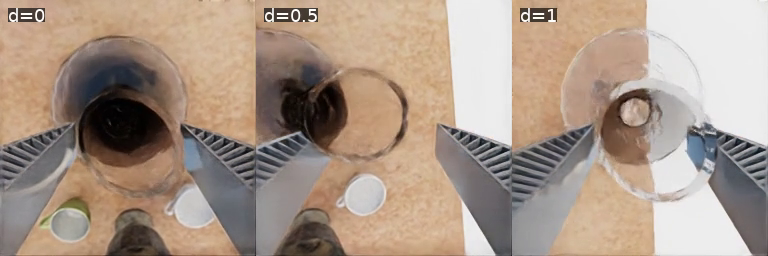
\includegraphics[width=\linewidth]{frames/task_0029-base-seed2002-wrist-t18s.png}
\caption{Historical native wrist frames at the same 18-second timestamp, columns
identity, midpoint and full dial. Top: full strength later completes safely while
the other settings time out. Bottom: both adapted settings violate uprightness;
full strength later completes unsafely. Selection is post hoc and illustrative.
The complete eight-block gallery and newly saved local matched videos retain the
positive and adverse context. No alternate trajectory is synthesized.}
\Description{Two three-panel strips illustrate one successful full-dial episode
and one adverse comparison from the original physical pilot.}
\label{fig:video}
\end{figure}

\section{Discussion and the next controlled comparison}
The evidence supports a direction-preserving implementation and identifies the
original trigger's lack of opportunity. It does not yet support a safe-execution
improvement. The sparse .04 rad intervention rate also means that a physically
inconclusive next screen is plausible. The proposed repair should therefore be
judged by observable controller behaviour first, and by complete outcomes second,
without changing caps or thresholds until a desired sign appears.

The recovery plan's smallest physical screen is eight full episodes: two
preselected development tasks crossed with identity, componentwise uniform cap/8,
vector cap/8, and vector cap with active refresh. All share the same cap and frozen
policy. The cap and threshold must be fixed before those outcomes; the sparse
threshold support above must remain disclosed. The screen is a mechanism test,
not a powered safety or optimizer comparison. A later timing-efficiency claim
also needs fixed-four/fixed-eight and a query-allowance control with actual query
counts, all costed in advance.

Evolutionary value requires the next comparison to include matched random search
and episodic ordinary learning over the same categorical controller and information.
The recovery plan proposes a categorical REINFORCE-style update with a baseline,
entropy regularization and fixed learning rate. These ordinary-learning updates
have not been implemented or run in this check-in. Copied elites and forced
identity anchors cannot be treated as uncorrected score-function samples.
All methods must receive the same shared initial data, descendant evaluation
allowance and confirmation cases, with finalists frozen before independent audit.
One optimizer seed would still support only a pilot.

The principal inferential limitation is the task denominator. Repeated frames,
prefixes and episodes within a small number of scenes are correlated. We do not
substitute them for independent task or optimizer-seed replication. Even zero
violations in eight independent homogeneous trials would have an approximate
95\% upper rate bound of $3/8=37.5\%$; repeated-scene dependence further limits
that illustrative calculation. No safety noninferiority claim follows from an
absence of a significant difference.

\section{Reproducibility and current status}
The repository retains the original frozen protocols, controller exports, public
attempt ledgers, native outcome audits and complete historical video galleries.
Private raw recordings and checkpoint lineage are revision-pinned and hash-verified.
The new recovery protocol fixes input roles, cap domain, threshold derivation,
prefix eligibility, a ten-minute analysis limit and zero new physical allocation.
Its outputs include source snapshots, frozen numerical thresholds, per-episode
geometry/timing tables and a public diagnostic receipt. Plotting and typesetting
do not replay physics.

The check-in deliverables are this paper draft, the completed offline diagnostic,
the tested recovery controller and annotated historical videos. The original
eleven-page cumulative evidence report remains available separately. Physical
repair comparisons, new evolutionary runs, random-search/ordinary-learning controls,
fresh-task recovery evaluation and replicated optimizer evidence remain future work.

\section{Conclusion}
A compact evolutionary controller is inexpensive to represent, but its training
winner need not improve safe completion. The original dial comparison is adverse,
and the original adaptive trigger never refreshes early. The completed recovery
diagnostic verifies a precise geometry repair while revealing sparse timing support.
The next scientific result must come from executing that repair in a prospectively
fixed physical comparison, followed by matched optimizer controls and independent
evaluation. Current evidence provides a concrete implementation and a testable
mechanism, with its physical benefit still open.

\begin{acks}
This work is supervised by Geraud Nangue Tasse at the University of the Witwatersrand.
AI coding assistance was used for implementation, analysis, prose and typesetting.
All reported physical outcomes derive from recorded native simulator/monitor traces.
The new replay diagnostic is explicitly separate from those physical measurements.
Experimental pictures and videos use recorded native images; schematic figures are
labelled as such. The archived studies and original recorded outcomes are unchanged.
\end{acks}
\bibliographystyle{ACM-Reference-Format}
\bibliography{references}
\end{document}
